\section{Procedure}

As the setup's base the D8 laboratory diffractometer from Bruker-AXS is used.
In this diffractometer, which is called $\theta - \theta$ diffractometer, the X-ray tube and detector can be rotated around the probe.
The X-ray tube is made of a copper anode and runs on $35\, \unit{\milli \ampere}$ and $35\, \unit{\kilo \volt}$.
The first thing to do before starting a measurement is to set up and adjust the used apparatus properly. 
The following sections provide the needed information to do so and further describe what data are collected.

\begin{figure}
	\centering
	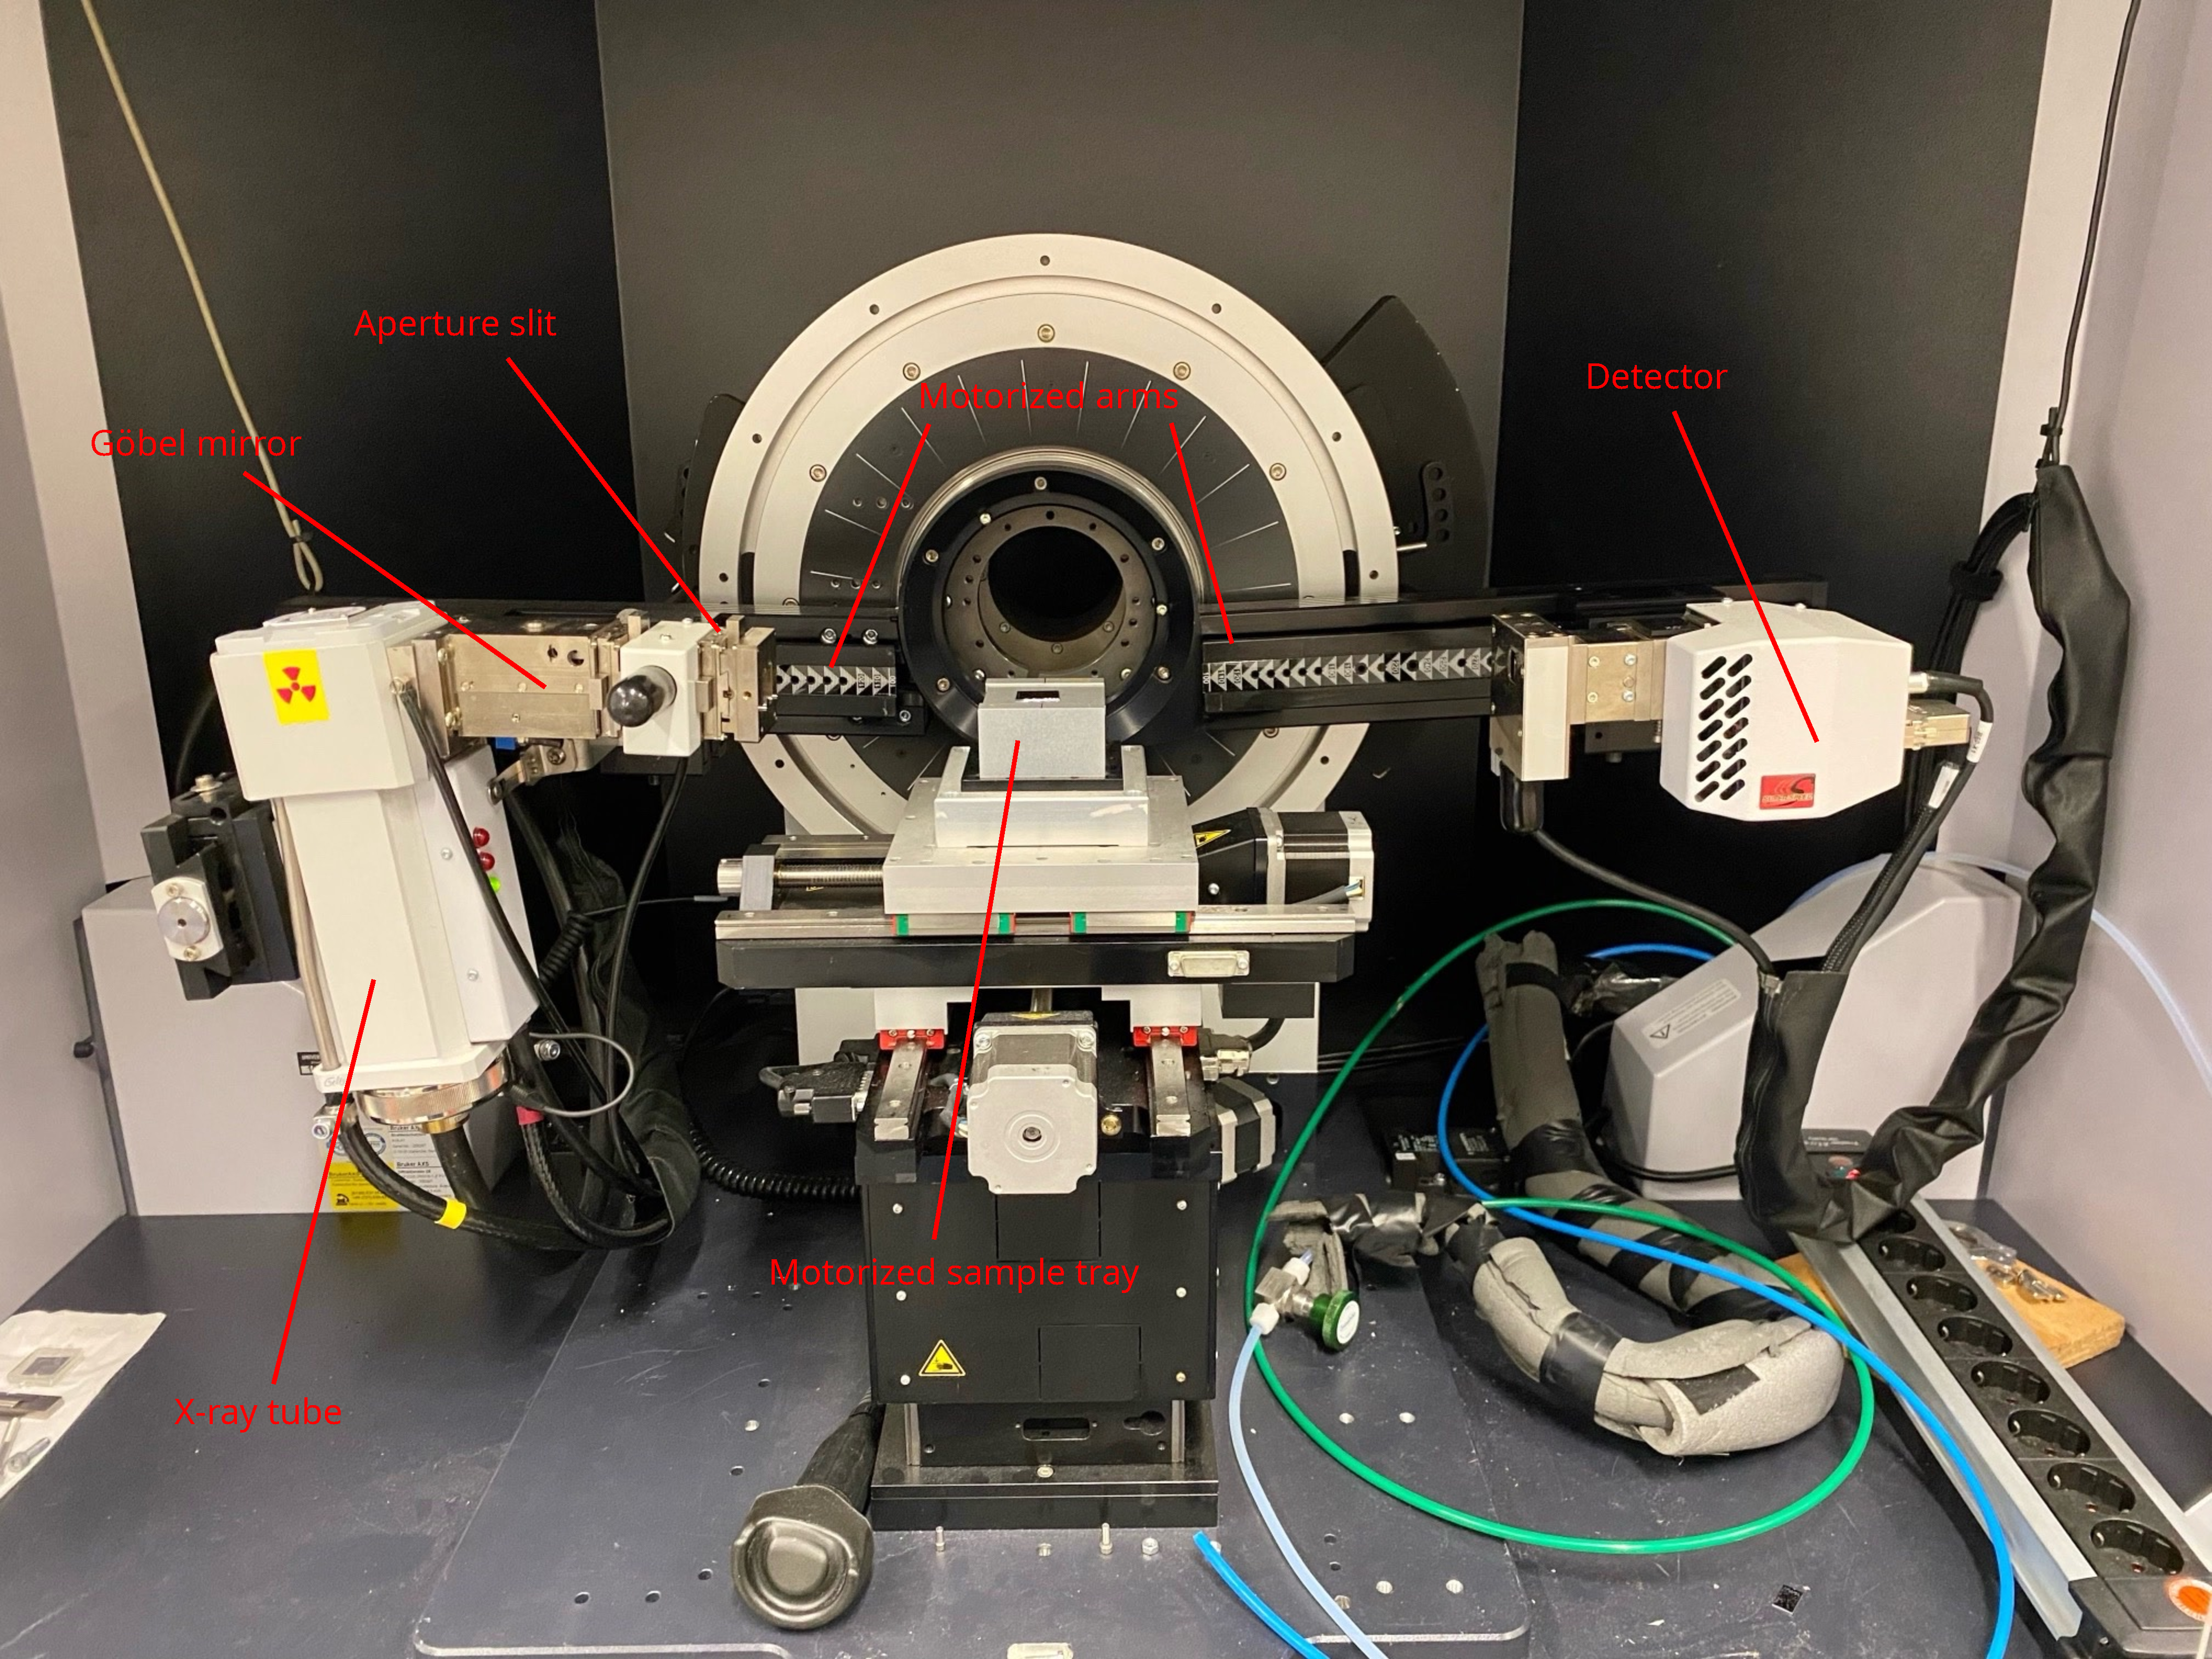
\includegraphics[width=0.55\textwidth]{content/graphics/apparatus.pdf}
	\caption{Appartus with labeled components.}
	\label{fig:Apparatus}
\end{figure}


\subsection{Adjustment of the D8 Diffractometer}
The XRD Commander program controls the diffractometer for adjusting the sample and collecting data. The most commonly used interface is the adjust mask. At the top, there is a toolbar with the MoveDrive, Init-Drive, and \textit{Zi} buttons, as well as a button to change the scales of the chart area. On the left side of the adjust mask are the Motor Drives Controls and Generator Controls. At the bottom are the Scan Controls.

To protect the detector from damage, the Absorber must first be set to Auto in the drop-down menu. Do not forget to press the Set button after selecting Auto. After activating the absorber, the geometry of the setup must be adjusted by positioning the X-ray beam, sample, and detector.

The position of the sample can be changed in X, Y, and Z directions using the Motor Drive Controls. Additionally, the position of the detector relative to the tube is changed by driving the 2θ motor. The motors are moved by typing the desired position into the Requested value field and setting the checkbox next to it. For example, to move the X-ray tube and the detector to position 0, you first type the value 0 in the corresponding field (2θ field) and set the checkmark on the right. In most situations, the program should set the corresponding checkmark by itself, so it does not have to be set manually. After pressing the Move-Drives button, the motors move to the desired position.

To measure reflectivity, the sample must be brought into the center of rotation of the diffractometer, and the sample surface must be aligned parallel to the X-ray beam. There are three available scan types: the Rocking Curve, the Detector Scan, and the Z-Scan. The measuring method can be selected via the Scantype drop-down menu at the bottom of the adjust mask. Additionally, the scanning ranges and the scan speed must be adjusted for each scan type. After performing the adjustment scans, the data should be saved in raw format, as it will be needed for later analysis.

At the beginning of the adjustment, the sample must be moved out of the beam by changing the Z-coordinate. Furthermore, both the tube and the detector must be moved to an angle of 0°.

\subsection{Adjustment of the primary beam}
The next thing to do is to adjust the primary beam. For this a detector scan, in which the detector moves in a small angular window around the beam's postion, is needed. 

As a result the intensity in dependency of the detector angle should behave like a Gaussian distribution. An example for this behaviour is shown in the top-left plot of \autoref{fig:Adjustplot}.

After measuring the distribution, the detectors zero position is set to be at the maximum of intensity. In order to save the new postion the so called \textit{Zi}-Button is clicked. By clicking the \textit{Zi}-Button the systems determines the centre of gravity of the peak and the zero position can then be exactly adjusted.
 
\subsection{Adjustment of the sample position}
Similar to the adjustment of the primary beam is the adjustment of the sample postion. By using the $X$, $Y$ and $Z$ coordinates the probe can be precisely placed in the beams centre. A good adjustment means that the probe is parallel to the beam and shades half of its intensity. 

The $Z$-axis is adjusted first. The height of the probe and the probe's shading can be changed by varying the $Z$ coordinate. If the intensity is at its maximum, the sample is below the beam. The $Z$ value for which the intensity is halved is estimated.

To properly align the sample along the X-axis, an X-scan is initially performed, resulting in a plateau of reduced intensity. This plateau allows flexibility in selecting an examination position on the sample. If adjustments to the sample’s X and Z positions yield an intensity of \( \frac{1}{2} I_{\text{max}} \), a rocking scan is then conducted to align the Y-coordinate (along the beam direction). 

During this scan, the X-ray tube and detector rotate around the sample, maintaining a constant angular sum \( i + f = 2 \), effectively rotating the sample within the beam. This rotation reveals any tilt of the sample relative to the X-ray beam and is also used to bring the sample's Y-axis to the diffractometer's center of rotation. Ideally, this measurement yields a symmetrical triangular peak in intensity. 

In practice, however, the triangle may appear asymmetrical, and the peak intensity may not occur exactly at \( \theta = 0 \). An asymmetrical triangle suggests that the beam does not strike the sample’s center (i.e., the sample is not centered in the rotation axis of the diffractometer). If, for example, the left side of the triangle is flatter than the right, the Y-coordinate should be increased; the reverse adjustment applies otherwise.

In cases where the rocking scan produces a plateau rather than a peak, this indicates misalignment in \( Z \) and excessive tilting of the sample. Once the triangle is symmetrical, double-clicking on the maximum intensity value determines its position and sends it to the motors. Using the "Move-Drives" option, the motors adjust to the new positions.

At this point, the X-ray tube and detector are set to the position where the rocking scan identified maximum intensity. This position is typically not exactly at \( \theta = 0 \). Due to the parallel alignment of the X-ray beam, the sample is no longer perfectly centered within the beam. Thus, a new Z-scan is necessary to re-center the sample to half the beam shading.

Next, a second rocking scan is performed at an angle of \( 2\theta = 0.3^\circ \) to further refine the sample alignment within the beam. If a clear reflection is visible, the angle of incidence and emergence can be set to \( 0.15^\circ \) by pressing the \textit{Zi} button and entering \( 0.15 \) in the theoretical position field.

Finally, a third Z-scan can refine the half-shading position by locating the maximum of the intensity curve, indicating the complete reflection of the primary beam within a particular height range \( Z \). At this point, an angled Z-scan is conducted \autoref{fig:zscan}. The scan range should be close to zero, and the maximum intensity is selected by double-clicking the curve’s center of gravity and moving to the corresponding \( Z \)-position. For finer adjustments, a final rocking scan is performed at \( 2\theta = 0.5^\circ \), using the \textit{Zi} key and entering \( 0.25 \) in the theoretical position input field to calibrate the angles of incidence and reflection.


\begin{figure}
	\centering
	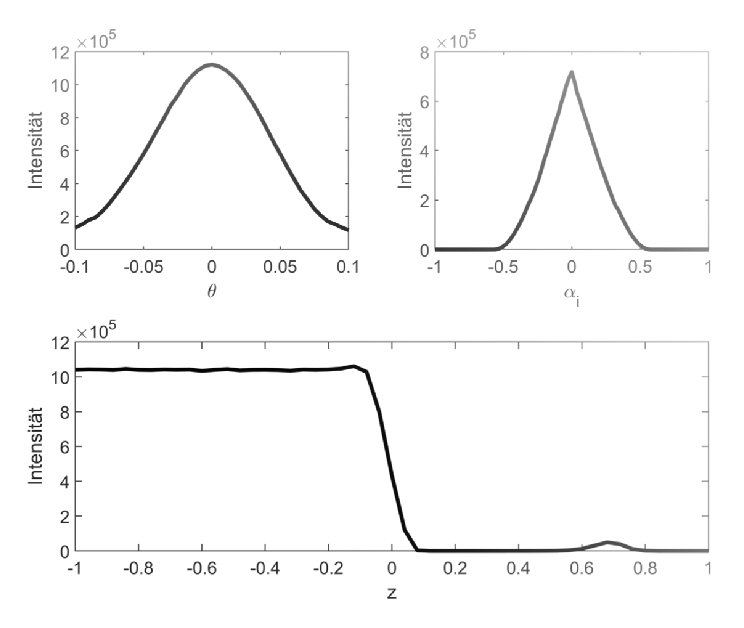
\includegraphics[width=0.66\textwidth]{content/graphics/AdjustmentPlots.pdf}
	\caption{Example measurements of different scantypes needed for the proper adjustment of the apparatus. Top left: Detector scan for beam adjustment, Top right: Rockingscan for $Y$-axis adjustment, Bottom: Z-Scan for sample position \cite{xray}. }
	\label{fig:Adjustplot}
\end{figure}

\begin{figure}
	\centering
	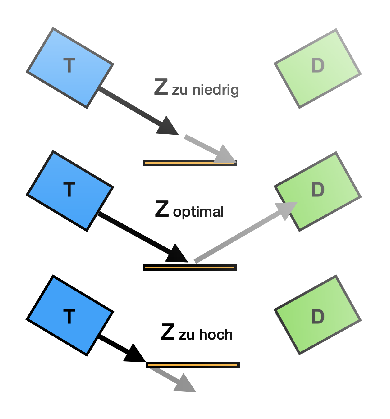
\includegraphics[width=0.33\textwidth]{content/graphics/zscan.pdf}
	\caption{Z-Scan for $2\theta = 0.3°$ \cite{xray}.}
	\label{fig:zscan}
\end{figure}

Every additional information needed for the measurements is shown in \autoref{fig:tableAdj}.
\begin{figure}
	\centering
	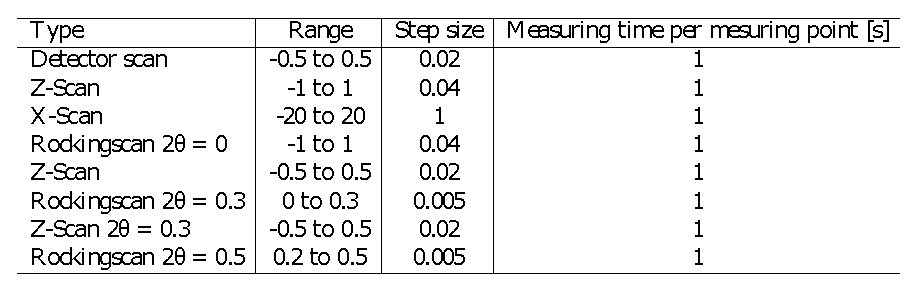
\includegraphics[width=0.66\textwidth]{content/graphics/table.pdf}
	\caption{Table with additional information for the adjustment \cite{xray}.}
	\label{fig:tableAdj}
\end{figure}

\subsection{Measurement of polymer coated silicon wafer}

Now the actual measurement of the silicon wafer can start. The angles of incidence (\( i \)) and detection (\( f \)) are equal for this scan, which uses the Omega/2Theta scan type. A scan range from \( 0^\circ \) to \( 25^\circ \) can be selected with a recommended step width of \( 0.005^\circ \) and a measuring time of at least 5 seconds per step.

To obtain the true reflectivity, a diffuse scan, which measures scattered radiation, must also be performed. For this scan, the detector angle is offset by \( 0.2^\circ \) relative to the incidence angle, using the same step size. All data should be saved in raw format, converted with the program File Exchange, and stored on a USB stick. This completes the measurement process, and the data are ready for analysis.

For smaller angles $\alpha_i$ the beam can be wider than the sample resulting in lower intensities. Its useful to define the angle $\alpha_g$ which is defined as the geometry angle at which the beam hits the whole surface of the wafer. For smaller angles a correction is needed. The intensity for $\alpha_i$ is expanded by $G=\frac{D\sin{\alpha_i}}{d_0}$ with the beam width $D\sin{\alpha_i}$ and the total beam width $d_0$.  
